\chapter{Data}
\label{ch:data}

GroundOne learns a single decision, so the data must teach exactly that decision and allow it to be measured
reliably. The chapter first defines the decision and its labels. It then describes the three public datasets from which
the labels come and the way they are turned into the training set, the dev set and the test sets. The last sections
show how the reliability of the test sets was verified without new annotations, what an exploratory analysis of the
built dataset reveals and how leakage between training and test data was ruled out.

% Source of truth for every number in this chapter: Project/data/processed/groundone/DATACARD.md and
% build_report.json (dataset), Project/experiments/eda/report/eda_report.md and stats/ (exploratory analysis).

\section{Task and labels}
\label{sec:data-task}

The input consists of a retrieved document and an answer, written by a language model and split into sentences. For
every sentence the model decides whether, \emph{with respect to the document}, it is \emph{supported},
\emph{contradicted} or \emph{not mentioned}. A sentence is supported when the document states, or directly implies,
everything it asserts. It is contradicted when some part of it conflicts with the document. It is not mentioned when it
adds information that the document does not contain but does not contradict either. When a sentence contains both a
conflicting part and an unverifiable part, it is labelled as contradicted, because a contradiction is the more serious
error. Only the document counts: a statement that is true in the real world but absent from the document is still not
mentioned.

The number of decisions required by an answer equals the number of its scored sentences, denoted $K$. This quantity is
central to the thesis. A decision model reads the document and the answer only once, so each additional decision costs it little, only the tokens of the sentence and the three of its marker; an LLM judge, by contrast, has to produce text for every sentence. For this reason the
comparison with LLM judges is carried out as a function of $K$, and the data must include long answers as well
as short ones.

For every sentence the model returns three probabilities, and every other quantity is derived from them instead of
being learned separately. The binary groundedness score, used for the comparison with published binary benchmarks, is
$P(\text{supported})$. Flags, instead, depend on the notion of error adopted. Under a \emph{strict} policy, anything
the document does not state is an error, and a sentence is flagged when $P(\text{supported})$ falls below a threshold
$\tau$. Under a \emph{lenient} policy, only contradictions are errors, and a sentence is flagged only when it is judged
contradicted. In this way the user chooses the notion of error and the threshold at inference time, without retraining
the model. Section~\ref{sec:method-calibration} gives the exact rule with which the verifier produces the labels it
returns.

\section{Source datasets}
\label{sec:data-sources}

The dataset is deliberately built from as few sources as possible: one for training and three for testing
(Table~\ref{tab:data-sources}). With fewer sources, the definition of the labels and the text format remain unique, and
there are fewer points at which the construction can introduce errors.

\begin{table}[htbp]
\centering
\caption{The source datasets: licence, role in GroundOne and type of the original labels.}
\label{tab:data-sources}
\small
\begin{tabularx}{\textwidth}{@{}>{\raggedright\arraybackslash}p{0.25\textwidth}>{\raggedright\arraybackslash}p{0.18\textwidth}>{\raggedright\arraybackslash}p{0.15\textwidth}>{\raggedright\arraybackslash}X@{}}
\toprule
Dataset & Licence & Role & Labels \\
\midrule
RAGTruth~\cite{niu2024ragtruth} & MIT & Training set, dev set and test T1 & Character spans of LLM answers, annotated with four hallucination types (conflict or baseless information, evident or subtle). \\ \addlinespace
\mbox{LLM-AggreFact}~\cite{tang2024minicheck,llmaggrefact} & \mbox{CC BY-ND 4.0} & Test T2 only & One binary label per claim: supported or unsupported. \\ \addlinespace
VitaminC~\cite{schuster2021vitaminc} & \mbox{CC BY-SA 3.0} & Test T3 only & Three classes per claim: \emph{supports}, \emph{refutes} and \emph{not enough information}. \\
\bottomrule
\end{tabularx}
\end{table}

\paragraph{RAGTruth.} RAGTruth~\cite{niu2024ragtruth} contains 17{,}790 answers written by six language models
(GPT-3.5, GPT-4, Llama-2 7B, 13B and 70B, and Mistral-7B) in three RAG tasks, which differ in the type of context. In
question answering the context is a set of passages retrieved for an MS~MARCO question~\cite{nguyen2016msmarco}. In
summarisation it is a news article, taken from CNN/DailyMail~\cite{hermann2015teaching,see2017pointer} or from recent
news. In data-to-text generation, where the model describes structured data in prose, the context is the record of a
Yelp business in JSON format~\cite{yelpdataset}. In each answer, two trained annotators identified the character spans
not supported by the context\footnote{A \emph{span} is a contiguous stretch of text, identified by the positions of its
first and last characters. A span-level annotation marks the exact portion of the answer that contains the error,
instead of judging the answer as a whole.}, with a third review in cases of disagreement. They then assigned each span
one of four types: \emph{conflict}, evident or subtle, and \emph{baseless information}, evident or subtle. The paper
reports an inter-annotator agreement of 91.8\,\% at the answer level and 78.8\,\% at the span level. RAGTruth is the
only public dataset that combines natural multi-sentence answers, produced by different models, with the distinction
between contradicted and unsupported content, and for this reason it is the only training source. The official split
separates 450 test sources from the remaining ones, which are intended for training.

\paragraph{LLM-AggreFact.} LLM-AggreFact~\cite{tang2024minicheck,llmaggrefact} aggregates eleven manually annotated
fact-checking datasets, each made of (document, claim) pairs. The datasets cover three areas: summarisation
(AggreFact-CNN and XSum~\cite{tang2023aggrefact}, TofuEval~\cite{tang2024tofueval}, with its two subsets MediaS and
MeetB), retrieval-based or long-form question answering (RAGTruth~\cite{niu2024ragtruth},
ClaimVerify~\cite{liu2023verifiability}, ExpertQA~\cite{malaviya2024expertqa}, LFQA~\cite{chen2024lfqa}) and fact
checking proper (WiCE~\cite{kamoi2023wice}, REVEAL~\cite{jacovi2024reveal},
FactCheck-GPT~\cite{wang2024factcheckbench}). The benchmark has a public leaderboard, which makes the results comparable
with those of published systems. Its access condition, however, forbids using the data to train models~\cite{hf_llmaggrefact}.
In this thesis the dataset therefore serves only for evaluation: no training, calibration or selection takes place on
any of its splits.

\paragraph{VitaminC.} VitaminC~\cite{schuster2021vitaminc,hf_vitaminc} is a fact-verification dataset built from
Wikipedia revisions that change a fact. For each revision, trained annotators wrote claims supported by one version of
the sentence and refuted by the other. When no contradiction could be formulated, the pair was labelled as having not
enough information. The two versions of the evidence are almost identical, so to decide, a model must look at the
precise fact rather than at word overlap. On a re-annotated sample of 2{,}000 pairs the authors report a Fleiss'
$\kappa$ of 0.71\footnote{Fleiss' $\kappa$ measures the agreement among several annotators net of the agreement that
would be obtained by pure chance: it equals 1 when agreement is perfect and 0 when it does not exceed chance.}. In this
thesis VitaminC fills a precise gap. RAGTruth does not publish the inter-annotator agreement on the hallucination
\emph{type}, so on its own it cannot show that the model learns the boundary between contradicted and not mentioned.
VitaminC provides exactly this boundary, with labels of known reliability and in a different domain.

Several other candidates were examined and discarded. NLI corpora such as ANLI~\cite{nie2020anli} have short premises,
far from typical RAG contexts, and the same three-class distinction on factual text is already covered by VitaminC.
Synthetic or binary-only training data, such as the data released with MiniCheck~\cite{tang2024minicheck}, lack
three-class labels. Finally, datasets with labels generated by a language model and datasets that reuse RAGTruth test
answers were excluded: in this way the labels remain human and the test sets remain independent.

\section{Construction}
\label{sec:data-construction}

\paragraph{Sentence segmentation.} Answers often contain lists and headings, so they are first split at line breaks.
Each line is then divided into sentences with PySBD~\cite{sadvilkar2020pysbd}, a rule-based segmenter that handles
abbreviations and decimal numbers. Leading list markers, such as ``3.'' or ``*'', are removed, because they concern
layout and not content. The same segmenter is used in training, evaluation and inference, so that the model always sees
sentences cut in the same way. Figure~\ref{fig:data-pipeline} summarises the whole construction process, from the
sources to the frozen test sets.

\begin{figure}[htbp]
\centering
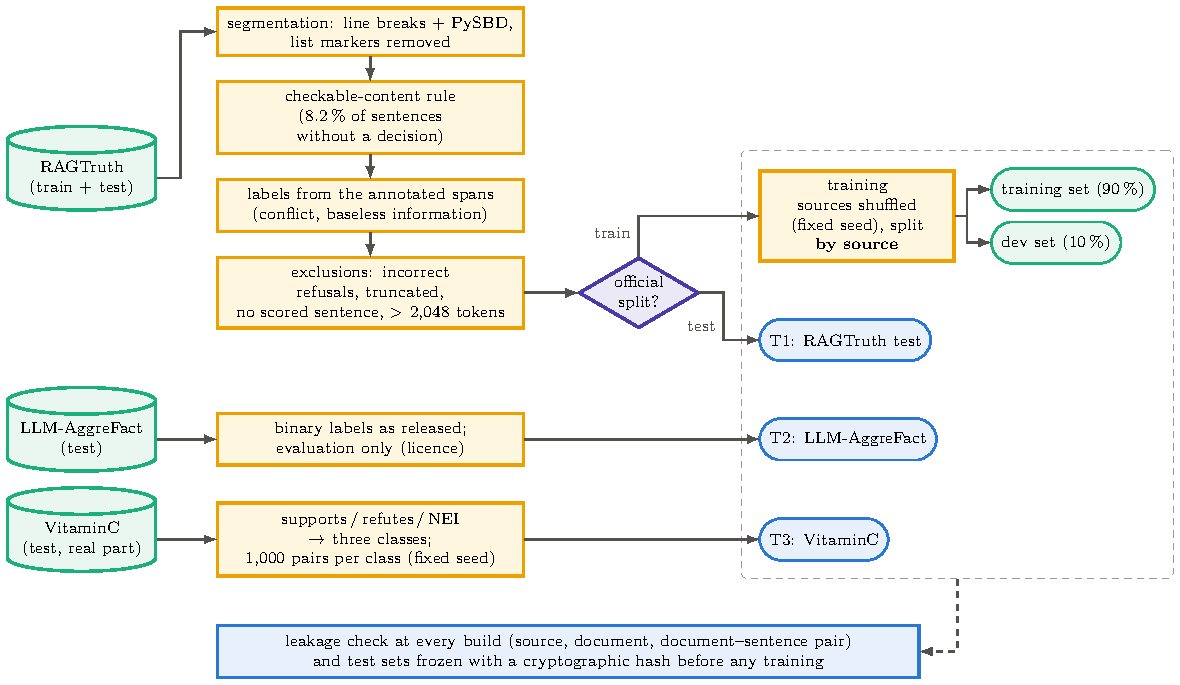
\includegraphics[width=\textwidth]{images/diagrams/data_pipeline_tikz.pdf}
\caption{Construction of the dataset. RAGTruth answers are segmented, filtered of sentences without checkable content, labelled from the spans and cleaned of exclusions; the official test split becomes T1, while the training sources are divided by source into training set and dev set. LLM-AggreFact and VitaminC provide only test sets (T2 and T3). An automatic leakage check accompanies every build, and the test sets are frozen with a hash before any training.}
\label{fig:data-pipeline}
\end{figure}

\paragraph{Sentences without checkable content.} Some sentences assert nothing about the document: greetings, headings
that introduce a list, lines containing only a citation, such as ``(Passage 2)'', and refusal formulas. These sentences
remain in the numbered answer as context, but they are not decisions and carry no label. A short rule identifies them,
and it applies to 8.2\,\% of all RAGTruth sentences, mostly list headings. The rule considers only the form of the sentence, that is, fewer than two words, a final colon, a line containing only a citation or a conversational or refusal formula, and it never changes a label. Its coverage was verified
against the independent segmentation of LLM-AggreFact, described in Section~\ref{sec:data-reliability}.

\paragraph{Labels.} In RAGTruth the label of a scored sentence depends on the spans it overlaps. The sentence is
contradicted if it overlaps a conflict span, not mentioned if it overlaps only baseless-information spans, and
supported in all other cases. Only 27 of the 14{,}226 annotated spans (0.19\,\%) touch no scored sentence, so the
conversion loses almost no annotation. For LLM-AggreFact, instead, the binary label is kept as released. VitaminC
labels are converted directly: \emph{supports} becomes supported, \emph{refutes} contradicted and \emph{not enough
information} not mentioned. Figure~\ref{fig:data-label-rule} summarises the rule applied to RAGTruth.

\begin{figure}[htbp]
\centering
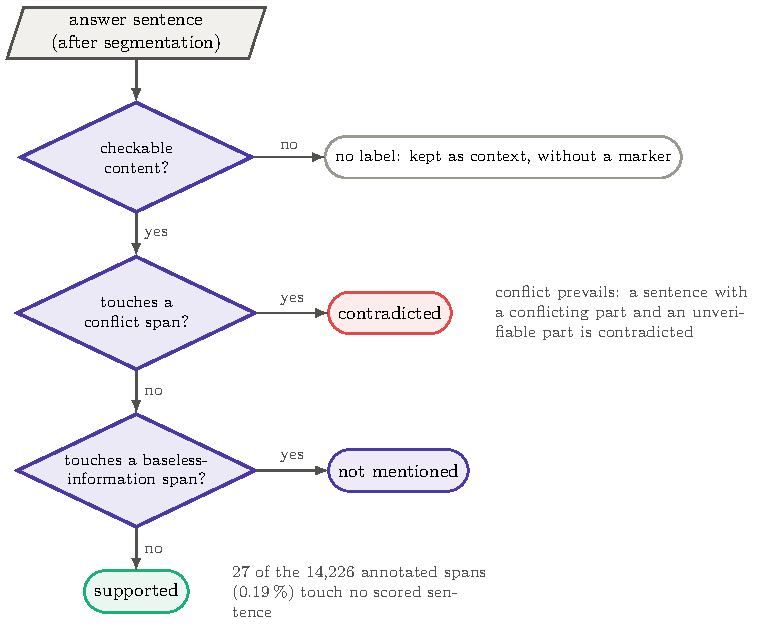
\includegraphics[width=0.85\textwidth]{images/diagrams/data_label_rule_tikz.pdf}
\caption{Rule by which the span-level annotations of RAGTruth become sentence labels. Sentences without checkable content remain in the prompt as context but are not decisions; among the others, conflict prevails over baseless information.}
\label{fig:data-label-rule}
\end{figure}

\paragraph{Exclusions and splits.} Three categories of answers are removed: those that RAGTruth flags as incorrect
refusals or as truncated, those without any scored sentence and those in which document, answer and the about 80 tokens of the prompt together exceed 2{,}048 tokens. This last length limit is imposed by the memory of the 16\,GB laptop. The official RAGTruth test split
becomes test set T1. The training sources, instead, are shuffled with a fixed seed and divided into two parts: 10\,\%
forms the dev set and the rest the training set. Since the division is made by source, answers about the same source
never appear in both sets. Six training answers about a news article that also appears in the LLM-AggreFact test set
are removed as well. Finally, the real (non-synthetic) part of the VitaminC test split is unbalanced across classes,
so T3 is formed by sampling from it, with a fixed seed, 1{,}000 pairs per class.

\section{The resulting dataset}
\label{sec:data-result}

Table~\ref{tab:data-splits} summarises the five files of the dataset. The training set contains 13{,}203 answers and
90{,}795 labelled sentences. Each record corresponds to an answer and contains one label for each sentence: in this
way the same data can feed different ways of reading the $K$ decisions of an answer.

\begin{table}[htbp]
\centering
\caption{The GroundOne dataset: number of records and of decisions by split and by class. A decision is a labelled
sentence. T2 has binary labels, so its contradicted and not-mentioned sentences are merged into the unsupported
class.}
\label{tab:data-splits}
\small
\begin{adjustbox}{max width=\textwidth}
\begin{tabular}{@{}llrrrrr@{}}
\toprule
Split & Source & Records & Decisions & Supported & Contradicted & Not mentioned \\
\midrule
Train & RAGTruth & 13{,}203 & 90{,}795 & 79{,}898 & 4{,}039 & 6{,}858 \\
Dev & RAGTruth & 1{,}468 & 9{,}996 & 8{,}827 & 410 & 759 \\
T1 & RAGTruth test & 2{,}647 & 17{,}284 & 15{,}745 & 584 & 955 \\
T2 & LLM-AggreFact test & 29{,}320 & 29{,}320 & 22{,}832 & \multicolumn{2}{c}{6{,}488 unsupported} \\
T3 & VitaminC test & 3{,}000 & 3{,}000 & 1{,}000 & 1{,}000 & 1{,}000 \\
\bottomrule
\end{tabular}
\end{adjustbox}
\end{table}

RAGTruth is strongly imbalanced: about 88\,\% of the labelled sentences are supported, and contradictions are only about 4\,\% (Figure~\ref{fig:data-balance}). This is the natural frequency of errors in model answers, and it is
preserved. The test set thus reflects what a verifier meets in practice, while the imbalance is handled during
training. T3 compensates by offering a test balanced across the three classes.

Answers contain on average 6.9 scored sentences in the training set and 6.5 in T1, with a maximum of 28 in the training set and 23 in T1
(Figure~\ref{fig:data-k}). To analyse the results as a function of length, T1 is divided into four bands of $K$: 756
answers with 1--4 sentences, 1{,}288 with 5--8, 497 with 9--13 and 106 with 14 or more. When a results cell contains
at most 30 sentences of a minority class, as happens for contradicted sentences in question answering and in answers with fourteen or more sentences, the value is reported but marked as indicative.

\begin{figure}[htbp]
\centering
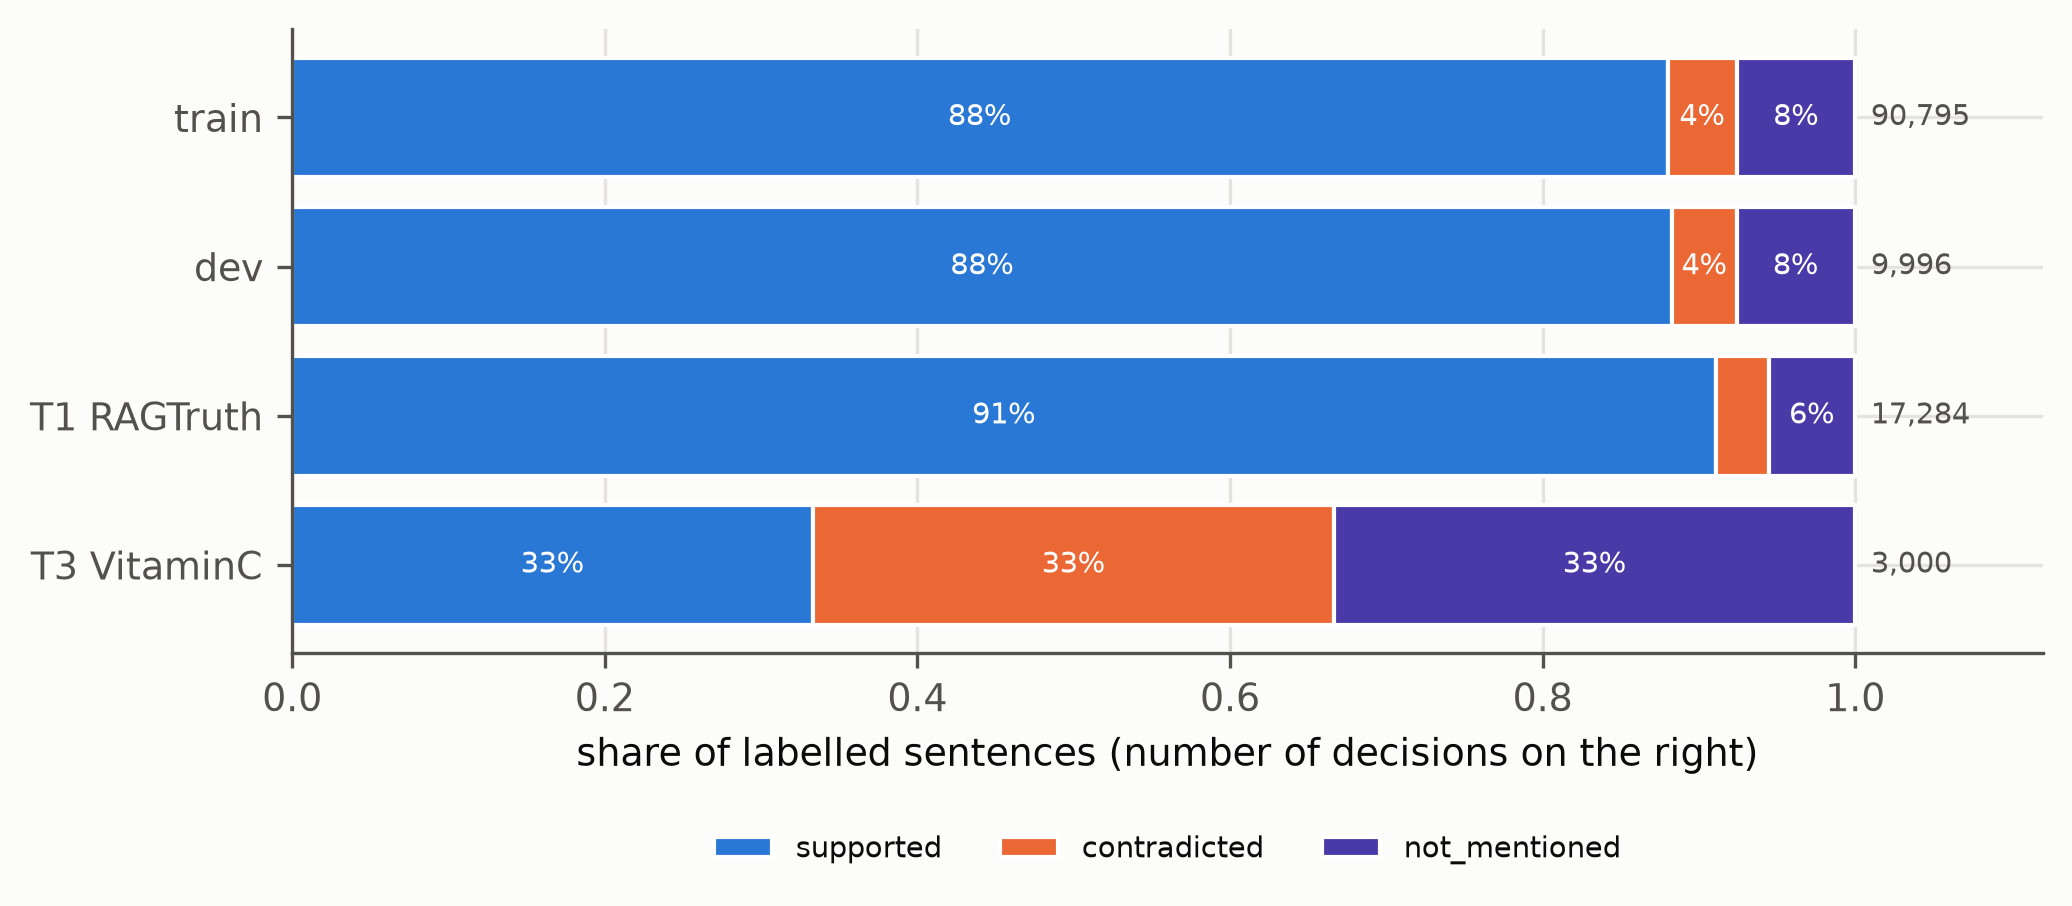
\includegraphics[width=0.9\textwidth]{images/dataset/class_balance_by_split.png}
\caption{Class distribution among the labelled sentences of each split. In the RAGTruth splits (train, dev and T1)
about 88--91\,\% of the sentences are supported. T2 (LLM-AggreFact) has binary labels, so its contradicted and
not-mentioned claims form a single unsupported class (hatched). T3 is sampled with 1{,}000 pairs per class.}
\label{fig:data-balance}
\end{figure}

\begin{figure}[htbp]
\centering
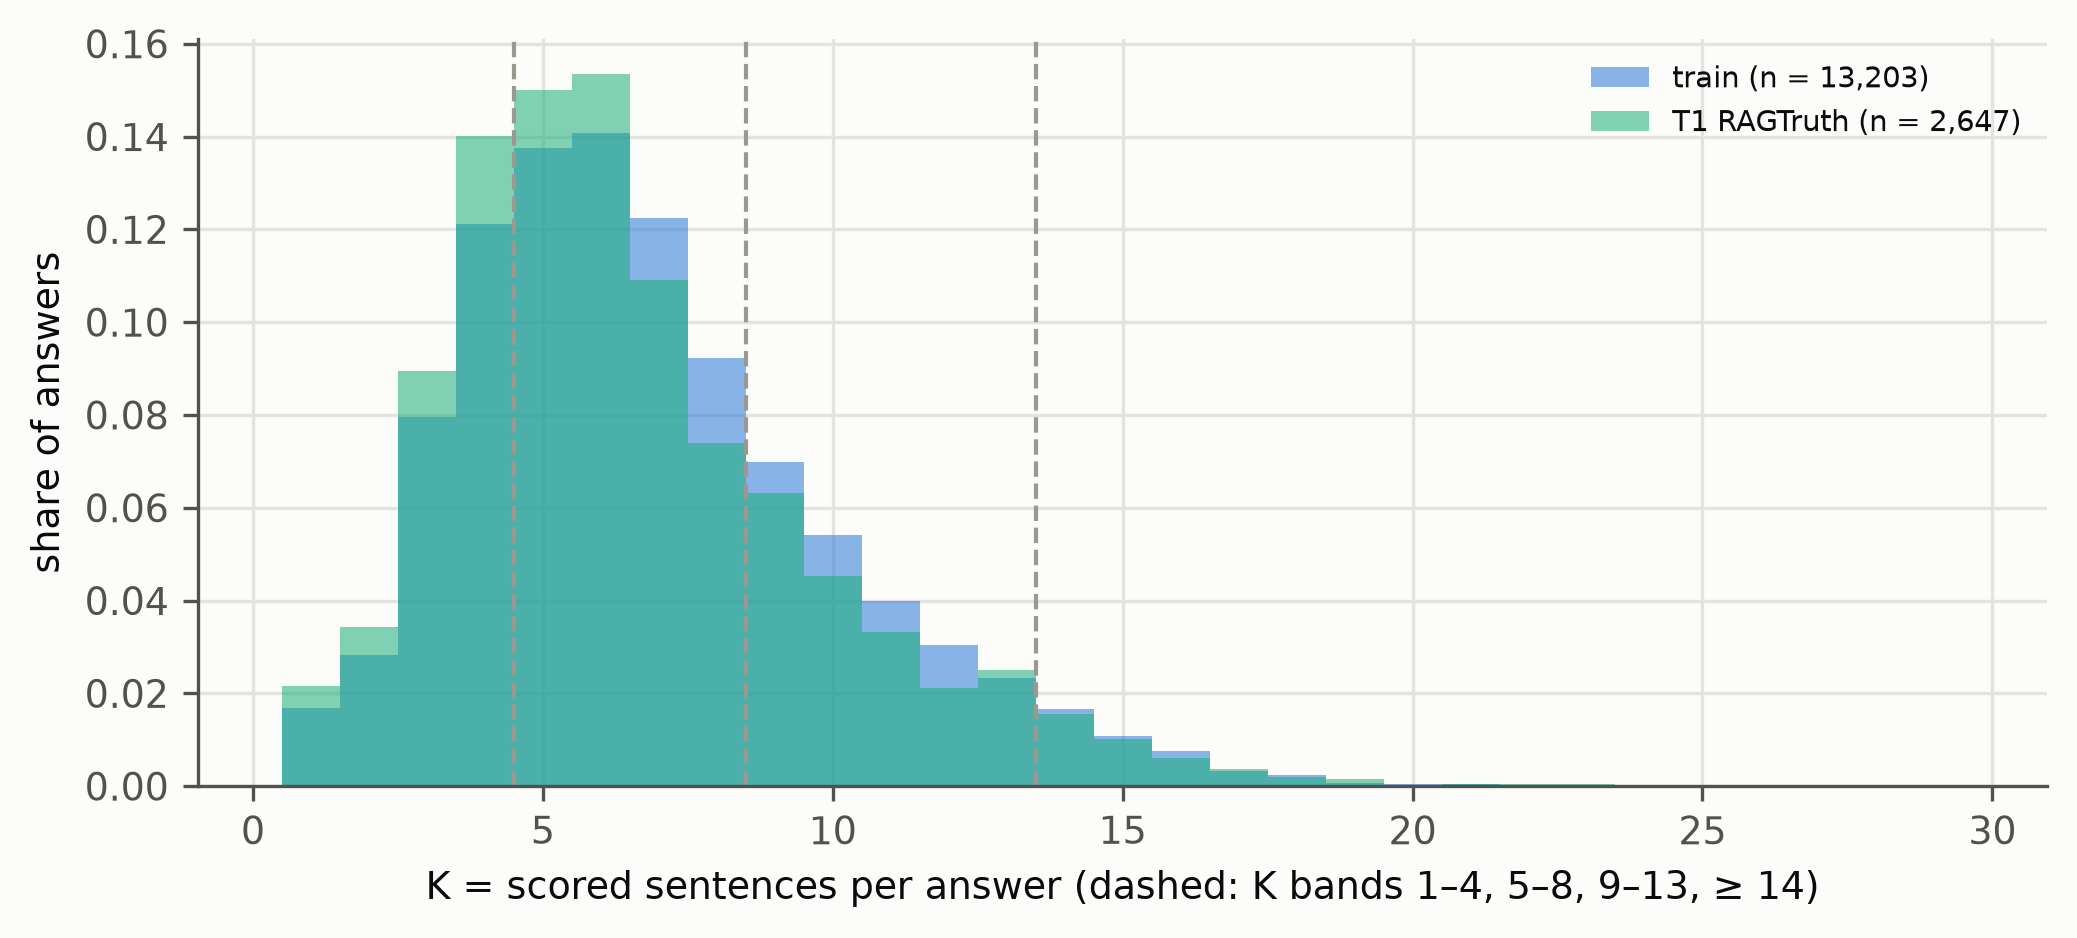
\includegraphics[width=0.9\textwidth]{images/dataset/K_distribution.png}
\caption{Distribution of $K$, the number of scored sentences per answer, in the training set and in T1. Dashed lines
delimit the bands of $K$ used to report the results.}
\label{fig:data-k}
\end{figure}

\section{Reliability of the test sets}
\label{sec:data-reliability}

The test sets were verified without new annotations, using evidence independent of the construction described above
(Table~\ref{tab:data-checks}). All test labels come from the human annotators of the published datasets. The two
choices that could introduce errors are segmentation and the conversion from spans to sentence labels. Both were
compared with LLM-AggreFact, whose authors independently converted the same RAGTruth test answers into sentence-level
claims. The segmenter of this thesis recovers exactly 96.3\,\% of their claims, and only 8.5\,\% of the scored
sentences are absent from their set. These are mostly sentences removed by their filter of ``non check-worthy''
claims, which is undocumented. On the 15{,}492 sentences present in both sets, the binary labels agree in 98.75\,\% of
cases. Moreover, all 193 disagreements go in the same direction: the span-based rule marks as unsupported a sentence
that LLM-AggreFact considers supported. Finally, an encoder-based baseline, evaluated on T2 without changes, reproduces
the score published by its authors (balanced accuracy of 74.0 measured, against 73.5 published), which validates the
evaluation code.

\begin{table}[htbp]
\centering
\caption{Reliability checks run before the test sets were frozen, with the pass criterion and the outcome of each.}
\label{tab:data-checks}
\small
\begin{tabularx}{\textwidth}{@{}lXl@{}}
\toprule
Check & Criterion & Outcome \\
\midrule
Label provenance & Every test label comes from human annotators. & Passed \\
Segmentation & At least 90\,\% of the LLM-AggreFact claims recovered among the segmented sentences, and at most 10\,\% of the segmented sentences absent from LLM-AggreFact. & 96.3\,\% and 8.5\,\% \\
Label derivation & Agreement of at least 97\,\% with the binary labels of LLM-AggreFact. & 98.75\,\% \\
Reference baseline & MiniCheck-RoBERTa on T2 within 1.5 points of the published score. & 74.0 against 73.5 \\
Leakage & No source, document or (document, sentence) pair shared between training and test. & Passed \\
\bottomrule
\end{tabularx}
\end{table}

These checks validate the binary side of T1, that is, the distinction between supported and unsupported sentences. The
distinction between contradicted and not mentioned rests instead on the RAGTruth annotators, whose agreement on the
hallucination type is not published. In addition, a recent re-annotation of the RAGTruth test split found 1.68 times
more hallucinated answers than the original labels~\cite{yu2026retromorphic}, which suggests that T1 underestimates the
two minority classes. For these reasons the three-class results on T1 are always read together with those on T3.

The content of the three test files was fixed when the dataset was built, after these checks and before any model was
trained, and recorded with cryptographic hashes\footnote{A cryptographic \emph{hash} is a fixed-length fingerprint computed from the content of a
file. Even a minimal change to the file produces a completely different fingerprint, so comparing fingerprints is
enough to detect any change.}. The files were then frozen: the hashes recorded at freezing time are identical to those
of the build. From that moment on, the program that generates the dataset from the raw sources (the
build command of the GroundOne package, Section~\ref{sec:method-software}) compares every new test file with its
fingerprint and refuses to overwrite it if the content has changed. Moreover, rerunning the build from scratch yields
exactly the frozen files: the test sets therefore cannot be modified, not even by mistake, after the results have been
seen.

\section{Exploratory analysis}
\label{sec:data-eda}

An exploratory analysis of the sources and of the built dataset brought to light four properties that affect how the
results are read.

\paragraph{Errors depend on the task and on the model.} Data-to-text answers contain hallucinations two to four times
as often as those of the other two tasks. The generator matters too: the answers of Llama-2 and Mistral account for
most of the hallucinations, while those of GPT-3.5 and GPT-4 are almost always faithful to the document
(Figure~\ref{fig:data-generators}). For this reason the results are reported task by task: a single average would
mostly reflect data-to-text.

\begin{figure}[htbp]
\centering
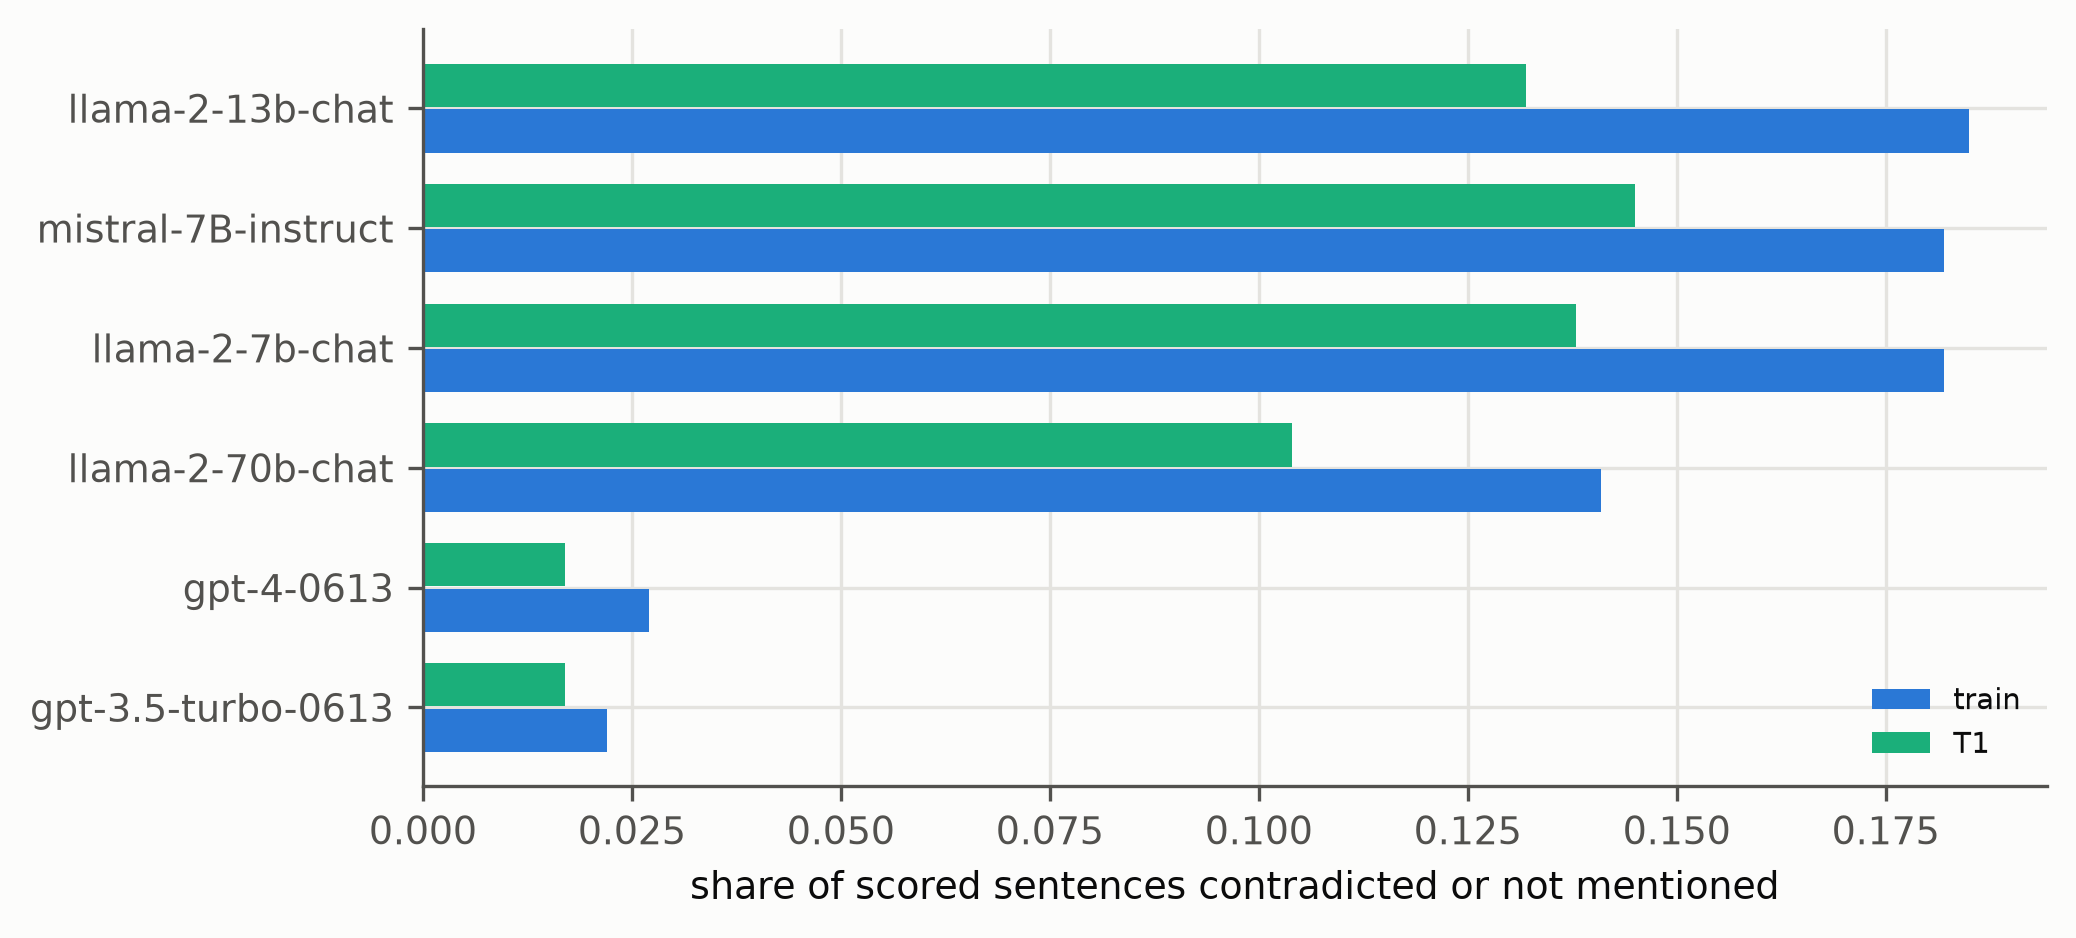
\includegraphics[width=0.9\textwidth]{images/eda/unsupported_by_generator.png}
\caption{Share of contradicted or not-mentioned sentences by the model that wrote the answer, in the training set and
in T1.}
\label{fig:data-generators}
\end{figure}

\paragraph{The test answers are cleaner than the training answers.} In every task and for every generator, the share
of contradicted and not-mentioned sentences is lower in T1 than in the training set. In question answering, for
example, 0.6\,\% of the T1 sentences are contradicted, against 1.6\,\% of those in the training set. As a consequence,
the metrics that depend on the base rate of the classes, such as precision or F1 on the minority
classes\footnote{The \emph{precision} of a class is the share of the predictions of that class that turn out to be
correct, and for this reason it changes with the frequency of the class even when the model stays the same. F1 is the
harmonic mean of precision and recall.}, are
not comparable between dev set and test set, because the dev set, drawn from the training set, preserves its
distribution. The primary metrics are therefore balanced accuracy, per-class recall and AUROC, which do not depend on the
base rate.

\paragraph{Contradictions are mostly evident.} About 85\,\% of the contradicted sentences of the training set come from
spans annotated as \emph{evident} conflicts, for example wrong numbers or names, while only 147 come from \emph{subtle}
conflicts. The contradicted class therefore consists mainly of blatant contradictions, and subtle contradictions cannot
be evaluated separately.

\paragraph{Surface cues exist, and they define the baselines.} Two simple cues predict the labels without verifying the
sentence against the document. The first is word overlap, that is, the share of the sentence's content words that also
appear in the document; content words are those that remain after excluding function words, such as articles,
prepositions and auxiliary verbs. In all three test sets this share is higher for supported sentences than for
contradicted and not-mentioned ones (Figure~\ref{fig:data-overlap}). Used on its own as a score, it separates supported
from unsupported sentences with an AUROC of 0.74 on T1 and 0.70 on T3. The second cue is the wording of the sentence.
In data-to-text, a classifier that sees only the sentence reaches a three-class balanced accuracy of 0.66, because in
Yelp descriptions some details are often invented, such as the number of reviews or the availability of Wi-Fi or valet
parking. In question answering and summarisation, instead, the same classifier stays at chance level (0.36 and 0.35),
and the same happens on T3 (0.33), where the contrastive construction of the dataset removes the cue. A verifier is
useful only to the extent that it beats these cues, so both are reported as baselines, task by task.

\begin{figure}[htbp]
\centering
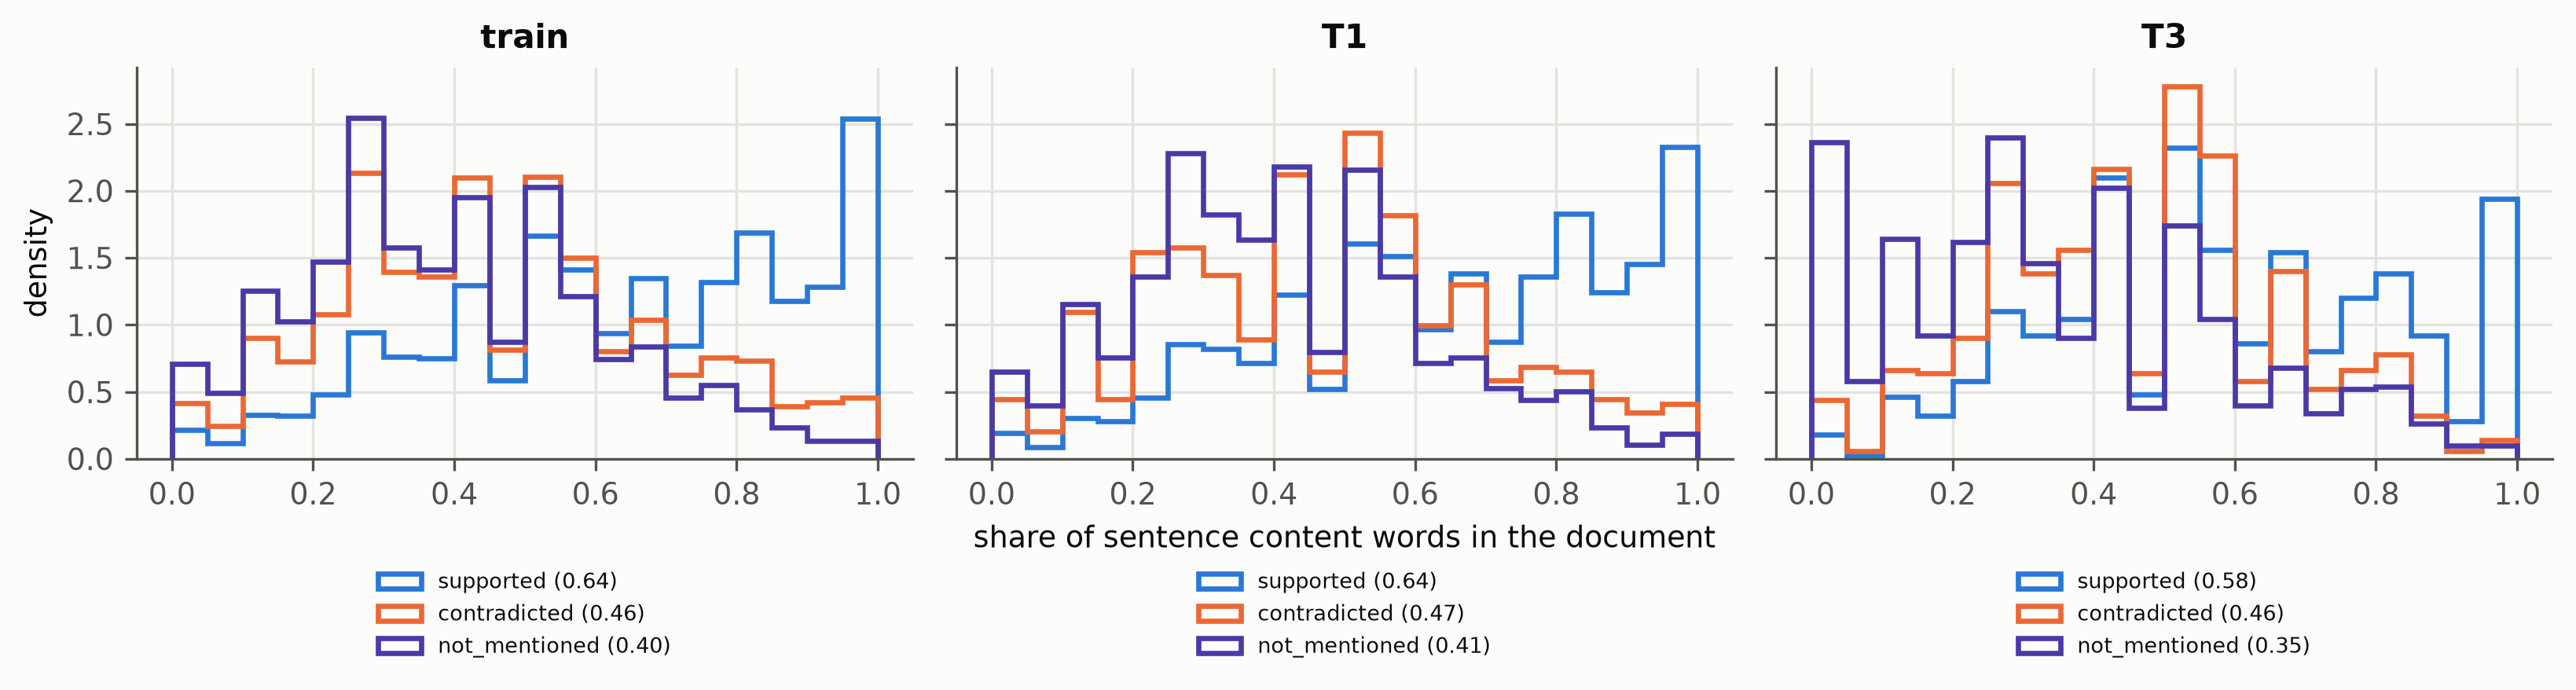
\includegraphics[width=\textwidth]{images/eda/overlap_by_class.png}
\caption{Word overlap between a sentence and its document, that is, the share of the sentence's content words present
in the document, by class, in the training set, in T1 and in T3. The mean is given in brackets.}
\label{fig:data-overlap}
\end{figure}

Finally, unsupported sentences are not concentrated at the end of the answer. The first sentence is rarely unsupported,
while the share of unsupported sentences peaks between the third and the fifth position and stays between 8 and
11\,\% in later positions (Figure~\ref{fig:data-position}). Long answers, too, therefore contain errors towards the end,
and accuracy at high values of $K$ remains relevant.

\begin{figure}[htbp]
\centering
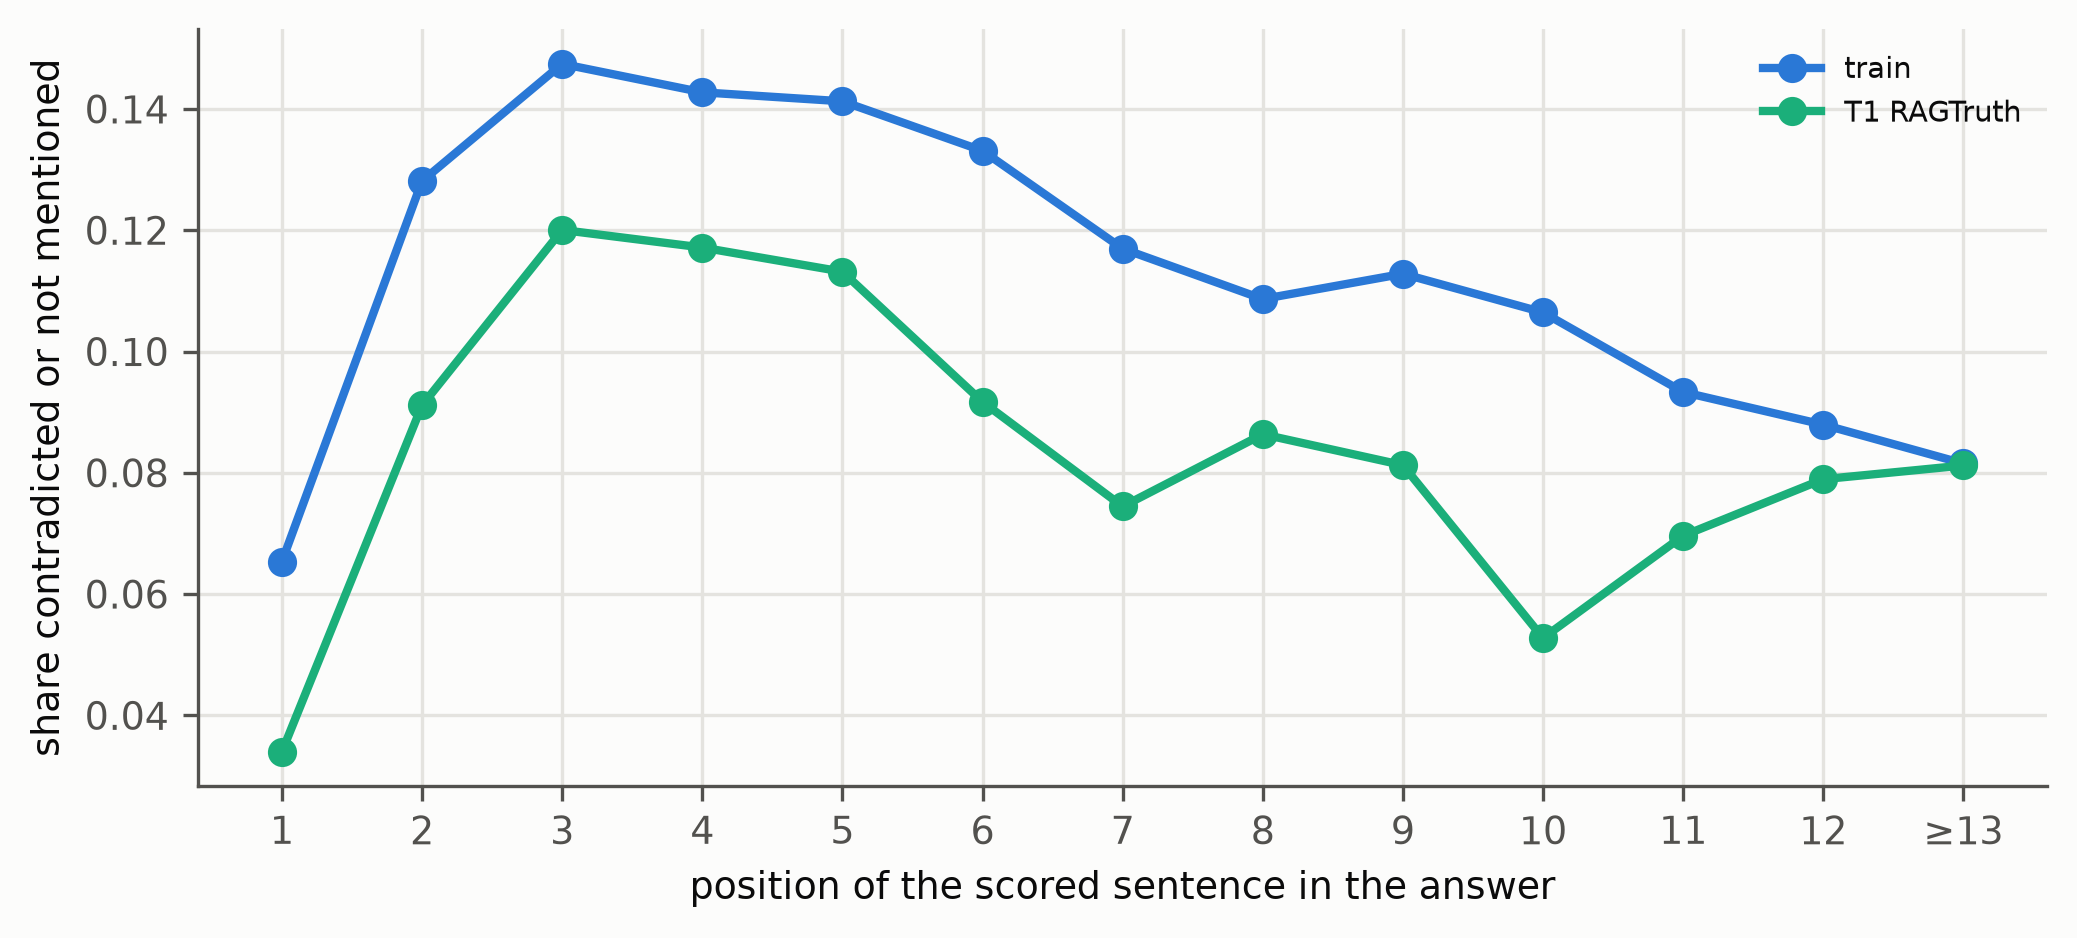
\includegraphics[width=0.9\textwidth]{images/dataset/unsupported_by_position.png}
\caption{Share of contradicted or not-mentioned sentences by the position of the sentence in the answer.}
\label{fig:data-position}
\end{figure}

\section{Leakage control}
\label{sec:data-leakage}

Leakage, that is, the presence of test-set information among the training data, would make all the metrics of the
following chapters optimistic. In this dataset the risk is concrete: RAGTruth contains, for every document, several
answers written by different models. If these answers ended up in different splits, the model would see in training
the very document on which it is later evaluated. For this reason the splits are defined by source and never by
sentence, so that all answers about the same source fall into the same split. In addition, an automatic check runs at
every build of the dataset, and it fails in two cases: when a source, a document or a (document, sentence) pair of the
training set or of the dev set appears in any of the test sets, and when the dev set and the training set share a
source. On the final dataset the check found no overlap of this kind. Without blocking the build, the check also lists
the sentences that appear with the same words in both training and test data, but refer to different documents. There are 788 in the training set and 82 in the dev set. Most of them, 702 of the 788, are standard data-to-text sentences, such as ``The business has a rating of 4.0 stars.'': the generator model repeats them for different businesses, so their presence in the training data does not anticipate any test label, which always depends on the document the sentence refers to. The others are generic phrases or come from different news articles on the same event, which the check, based on identical documents, does not recognise as related; they are few, but the overlap between different articles on the same story is not controlled. One aspect remains that cannot
be verified: whether the public datasets used here were part of the pre-training data of Qwen2.5. This is a limitation
common to most work on public benchmarks.
